%File: formatting-instructions-latex-2026.tex
%release 2026.0
\documentclass[letterpaper]{article} % DO NOT CHANGE THIS
\usepackage{aaai2026}  % DO NOT CHANGE THIS
\usepackage{times}  % DO NOT CHANGE THIS
\usepackage{helvet}  % DO NOT CHANGE THIS
\usepackage{courier}  % DO NOT CHANGE THIS
\usepackage[hyphens]{url}  % DO NOT CHANGE THIS
\usepackage{graphicx} % DO NOT CHANGE THIS
\urlstyle{rm} % DO NOT CHANGE THIS
\def\UrlFont{\rm}  % DO NOT CHANGE THIS
\usepackage{natbib}  % DO NOT CHANGE THIS AND DO NOT ADD ANY OPTIONS TO IT
\usepackage{caption} % DO NOT CHANGE THIS AND DO NOT ADD ANY OPTIONS TO IT
\frenchspacing  % DO NOT CHANGE THIS
\setlength{\pdfpagewidth}{8.5in}  % DO NOT CHANGE THIS
\setlength{\pdfpageheight}{11in}  % DO NOT CHANGE THIS
%
% These are recommended to typeset algorithms but not required. See the subsubsection on algorithms. Remove them if you don't have algorithms in your paper.
\usepackage{algorithm}
\usepackage{algorithmic}
\usepackage{amsmath}
\usepackage{amssymb}
\usepackage{subcaption}
\usepackage{booktabs}
\usepackage{tabularx}
\usepackage{tikz}
\usetikzlibrary{positioning, shapes.geometric, arrows.meta, fit, backgrounds}

%
% These are are recommended to typeset listings but not required. See the subsubsection on listing. Remove this block if you don't have listings in your paper.
\usepackage{newfloat}
\usepackage{listings}
\DeclareCaptionStyle{ruled}{labelfont=normalfont,labelsep=colon,strut=off} % DO NOT CHANGE THIS
\lstset{%
	basicstyle={\footnotesize\ttfamily},% footnotesize acceptable for monospace
	numbers=left,numberstyle=\footnotesize,xleftmargin=2em,% show line numbers, remove this entire line if you don't want the numbers.
	aboveskip=0pt,belowskip=0pt,%
	showstringspaces=false,tabsize=2,breaklines=true}
\floatstyle{ruled}
\newfloat{listing}{tb}{lst}{}
\floatname{listing}{Listing}
%
% Keep the \pdfinfo as shown here. There's no need
% for you to add the /Title and /Author tags.
\pdfinfo{
/TemplateVersion (2026.1)
}

% DISALLOWED PACKAGES
% \usepackage{authblk} -- This package is specifically forbidden
% \usepackage{balance} -- This package is specifically forbidden
% \usepackage{color (if used in text)
% \usepackage{CJK} -- This package is specifically forbidden
% \usepackage{float} -- This package is specifically forbidden
% \usepackage{flushend} -- This package is specifically forbidden
% \usepackage{fontenc} -- This package is specifically forbidden
% \usepackage{fullpage} -- This package is specifically forbidden
% \usepackage{geometry} -- This package is specifically forbidden
% \usepackage{grffile} -- This package is specifically forbidden
% \usepackage{hyperref} -- This package is specifically forbidden
% \usepackage{navigator} -- This package is specifically forbidden
% (or any other package that embeds links such as navigator or hyperref)
% \indentfirst} -- This package is specifically forbidden
% \layout} -- This package is specifically forbidden
% \multicol} -- This package is specifically forbidden
% \nameref} -- This package is specifically forbidden
% \usepackage{savetrees} -- This package is specifically forbidden
% \usepackage{setspace} -- This package is specifically forbidden
% \usepackage{stfloats} -- This package is specifically forbidden
% \usepackage{tabu} -- This package is specifically forbidden
% \usepackage{titlesec} -- This package is specifically forbidden
% \usepackage{tocbibind} -- This package is specifically forbidden
% \usepackage{ulem} -- This package is specifically forbidden
% \usepackage{wrapfig} -- This package is specifically forbidden
% DISALLOWED COMMANDS
% \nocopyright -- Your paper will not be published if you use this command
% \addtolength -- This command may not be used
% \balance -- This command may not be used
% \baselinestretch -- Your paper will not be published if you use this command
% \clearpage -- No page breaks of any kind may be used for the final version of your paper
% \columnsep -- This command may not be used
% \newpage -- No page breaks of any kind may be used for the final version of your paper
% \pagebreak -- No page breaks of any kind may be used for the final version of your paperr
% \pagestyle -- This command may not be used
% \tiny -- This is not an acceptable font size.
% \vspace{- -- No negative value may be used in proximity of a caption, figure, table, section, subsection, subsubsection, or reference
% \vskip{- -- No negative value may be used to alter spacing above or below a caption, figure, table, section, subsection, subsubsection, or reference

\setcounter{secnumdepth}{0} %May be changed to 1 or 2 if section numbers are desired.

% The file aaai2026.sty is the style file for AAAI Press
% proceedings, working notes, and technical reports.
%

% Title

% Your title must be in mixed case, not sentence case.
% That means all verbs (including short verbs like be, is, using,and go),
% nouns, adverbs, adjectives should be capitalized, including both words in hyphenated terms, while
% articles, conjunctions, and prepositions are lower case unless they
% directly follow a colon or long dash
\title{Evolutionary HyperNet-InfoGAN Baselines for Controllable Synthetic Image Generation}
\author{
	%Authors
	% All authors must be in the same font size and format.
	Mark Nuppnau\textsuperscript{\rm 1},
	Khalid Kattan\textsuperscript{\rm 2},
	R.G. Reynolds\textsuperscript{\rm 1}\\
}
\affiliations{
	%Afiliations
	\textsuperscript{\rm 1}Wayne State University \\
	robert.reynolds@wayne.edu
	% If you have multiple authors and multiple affiliations
	% use superscripts in text and roman font to identify them.
	% For example,
	
	\textsuperscript{\rm 2} University of Michigan - Dearborn\\
	kkattan@umich.edu
	% J. Scott Penberthy\textsuperscript{\rm 3}, 
	% George Ferguson\textsuperscript{\rm 4},
	% Hans Guesgen\textsuperscript{\rm 5}
	% Note that the comma should be placed after the superscript
	
	%
	% See more examples next
}

\begin{document}
	\renewcommand{\bottomfraction}{0.5}
	\maketitle
	
	\begin{abstract}
		Synthetic medical data generation requires human-auditable control. It is important that latent factors are able to separate data-specific structures so clinicians can inspect, trust, and responsibly reuse synthetic samples. Building on prior evolutionary generator work \cite{b1}, an Evolutionary HyperNet-InfoGAN is developed in which Policy Gradients with Parameter-Based Exploration (PGPE) optimizes a compact HyperNetwork that emits the weights of a larger image generator, while a discriminator/Q-network is trained with backpropagation. This process creates a non-stationary adversarial setting in which evolutionary search must continually adapt, but in a far smaller and more structured parameter space than direct evolution of the full generator.
		
		This model is used to evaluate a shared baseline on the MNIST dataset (28x28 grayscale, 10 classes) and then on a grayscale-converted BloodMNIST dataset (28x28, 8 classes) with a shared-z protocol in which groups of samples share continuous noise while discrete codes vary. This setup enables the direct measurement of feature-space code separation ($r_{sense}$) and within-code variation ($r_{intra}$). When compared to a previous PGPE baseline that searched directly over a generator with more than 500k parameters, the HyperNetwork formulation yielded cleaner code allocation, substantially more stable late-stage training, and the ability to resolve early duplicate modes to distinct digits for better mode coverage.
		
		When applied to MNIST, the baseline approached full digit coverage with fewer duplicate-code failures than prior direct search. For BloodMNIST, the preliminary baseline results show partial disentanglement and class-consistent morphology, suggesting that HyperNetworks provide a practical intermediate step toward auditable, controllable synthetic medical image generation. These baselines motivate the next stage of this work that will employ a Cultural Algorithms (CA) as a meta-level controller in order to support adaptive fitness weighting and secondary search guidance within the PGPE framework.
	\end{abstract}
	
	% Uncomment the following to link to your code, datasets, an extended version or similar.
	%
	% \begin{links}
		%     \link{Code}{https://aaai.org/example/code}
		%     \link{Datasets}{https://aaai.org/example/datasets}
		%     \link{Extended version}{https://aaai.org/example/extended-version}
		% \end{links}
	
	\section{Introduction}
	Generative Adversarial Networks (GANs) \cite{b3} are difficult to train because adversarial dynamics can lead to instability, mode collapse, and brittle gradients. InfoGAN \cite{b2} is attractive in this setting because it encourages latent variables to capture disentangled, human-inspectable structure without supervision. This is especially relevant in healthcare, where synthetic data should be controllable and auditable rather than merely realistic.
	
	\begin{figure}[t]
		\centering
		\resizebox{0.98\columnwidth}{!}{%
			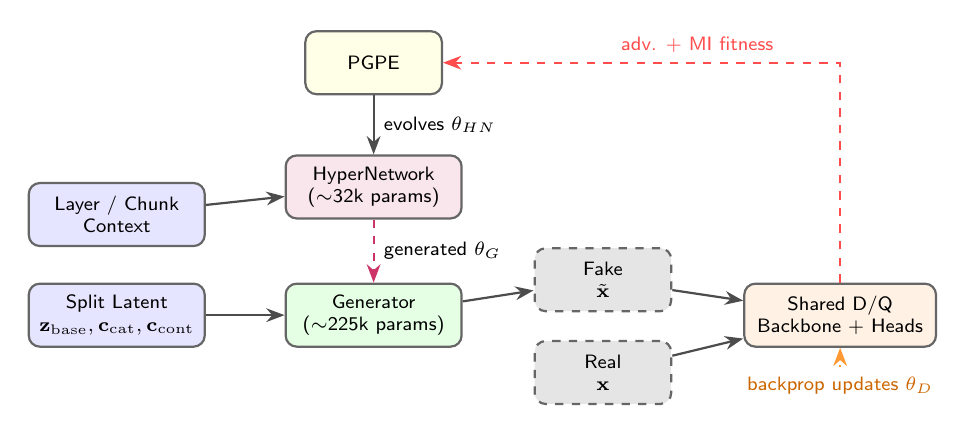
\begin{tikzpicture}[
				>=Stealth,
				font=\sffamily\scriptsize,
				node distance=0.6cm and 0.9cm,
				block/.style={
					rectangle, draw=black!60, rounded corners, thick,
					minimum height=0.8cm, text width=2.0cm, align=center
				},
				arrow/.style={->, thick, draw=black!70}
				]
				
				% Inputs
				\node[block, fill=blue!10] (context) {Layer / Chunk\\Context};
				\node[block, fill=blue!10, below=0.45cm of context] (latent) {Split Latent\\$\mathbf{z}_{\mathrm{base}}, \mathbf{c}_{\mathrm{cat}}, \mathbf{c}_{\mathrm{cont}}$};
				
				% Hypernetwork and generator
				\node[block, fill=green!10, right=1.0cm of latent] (gen) {Generator\\($\sim$225k params)};
				\node[block, fill=purple!10, above=0.8cm of gen] (hn) {HyperNetwork\\($\sim$32k params)};
				
				% Images and discriminator
				\node[block, fill=gray!20, dashed, text width=1.5cm, right=of gen, yshift=0.45cm] (fake) {Fake\\$\tilde{\mathbf{x}}$};
				\node[block, fill=gray!20, dashed, text width=1.5cm, below=0.35cm of fake] (real) {Real\\$\mathbf{x}$};
				\node[block, fill=orange!10, text width=2.2cm, right=of fake, yshift=-0.45cm] (disc) {Shared D/Q\\Backbone + Heads};
				
				% Optimizer
				\node[block, fill=yellow!10, above=0.75cm of hn, text width=1.5cm] (pgpe) {PGPE};
				
				% Forward path
				\draw[arrow] (context) -- (hn);
				\draw[arrow] (latent) -- (gen);
				\draw[arrow, draw=purple!80, dashed] (hn.south) -- node[right] {\scriptsize generated $\theta_G$} (gen.north);
				\draw[arrow] (gen) -- (fake);
				\draw[arrow] (fake) -- (disc);
				%\draw[arrow] (real.east) -- (disc.west |- real.east);
				\draw[arrow] (real) -- (disc);
				
				% Optimization signals
				\draw[arrow] (pgpe) -- node[right] {\scriptsize evolves $\theta_{HN}$} (hn);
				\draw[arrow, draw=red!70, dashed] (disc.north) |- node[above, pos=0.68, text=red!70] {\scriptsize adv. + MI fitness} (pgpe.east);
				
				% Backprop note for discriminator
				\node[below=0.25cm of disc, text=orange!80!black] (bpnote) {\scriptsize backprop updates $\theta_D$};
				\draw[arrow, draw=orange!80, dotted] (bpnote.north) -- (disc.south);
				
			\end{tikzpicture}
		}
		\caption{High-level baseline architecture. PGPE evolves a compact HyperNetwork ($\sim$32k parameters) that generates the full Generator parameter set ($\sim$225k parameters), reducing the dimensionality of evolutionary search.}
		\label{fig:architecture}
	\end{figure}
	
	In prior work \cite{b1}, generator backpropagation was replaced with PGPE \cite{b4}, to evolve the generator against a moving discriminator objective. While this avoided direct gradient propagation through the generator, it still required evolutionary search over a very large parameter space (more than 500k generator parameters), which often produced partial mode coverage and duplicated latent-code assignments. In the strongest MNIST runs, one class was typically missing and one or more codes collapsed to repeated digits.
	
\begin{figure*}[t]
	\centering
	
	\begin{subfigure}[t]{0.31\textwidth}
		\centering
		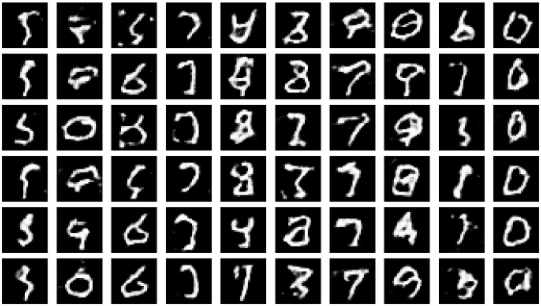
\includegraphics[width=\linewidth]{figures/mnist-0-21k.png}
		
		\vspace{0.5em}
		
		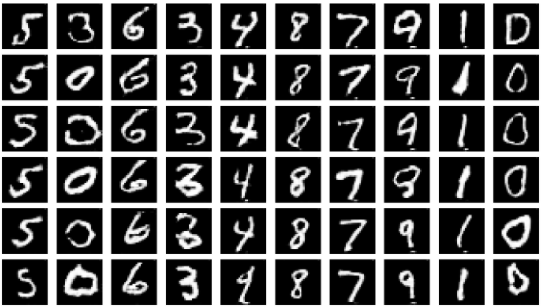
\includegraphics[width=\linewidth]{figures/mnist-0-198k.png}
		\caption{Direct encoding: duplicate `0' modes persist from 21k (top) through 198k (bottom).}
		\label{fig:mnist-0}
	\end{subfigure}
	\hfill
	\begin{subfigure}[t]{0.31\textwidth}
		\centering
		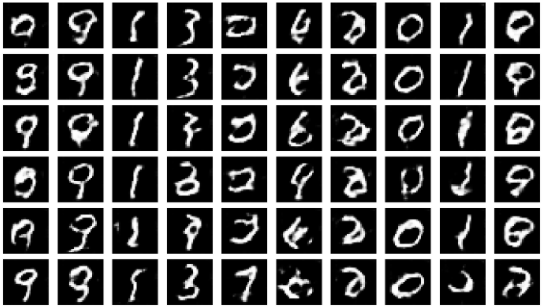
\includegraphics[width=\linewidth]{figures/mnist-1-21k.png}
		
		\vspace{0.5em}
		
		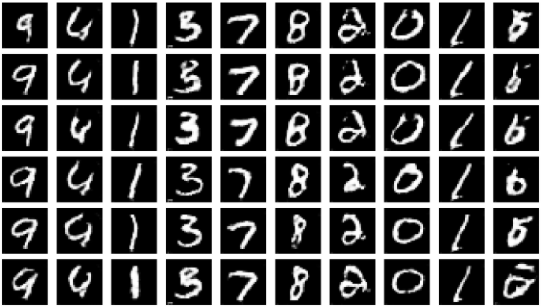
\includegraphics[width=\linewidth]{figures/mnist-1-198k.png}
		\caption{Direct encoding: duplicate `1' modes persist from 21k (top) through 198k (bottom).}
		\label{fig:mnist-1}
	\end{subfigure}
	\hfill
	\begin{subfigure}[t]{0.31\textwidth}
		\centering
		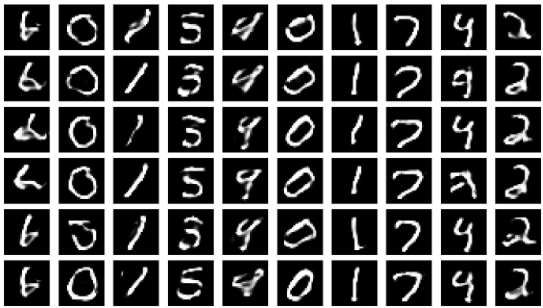
\includegraphics[width=\linewidth]{figures/mnist-hn-21k.png}
		
		\vspace{0.5em}
		
		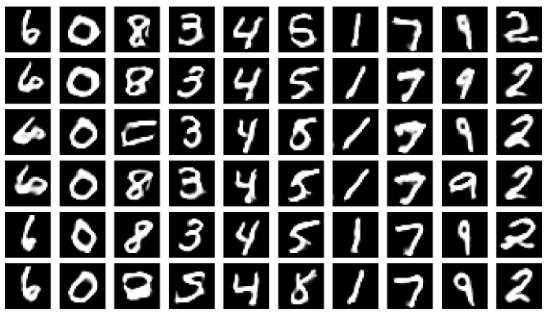
\includegraphics[width=\linewidth]{figures/mnist-hn-198k.png}
		\caption{Indirect encoding: duplicate `1' modes at 21k (top) resolve to distinct digits by 198k (bottom).}
		\label{fig:mnist-HyperNetwork}
	\end{subfigure}
	\caption{Mode duplication under direct vs.\ indirect encoding. Each panel shows 10 discrete codes (columns) at iteration 21k (top) and 198k (bottom). With direct encoding, PGPE searches over $>$500k generator parameters; duplicate modes that form early become permanent attractors (a,\,b). With indirect encoding via a hypernetwork ($\sim$32k parameters), the same duplicate modes appear early but are resolved during training, yielding full coverage of all 10 digit classes (c).}
	\label{fig:mode_resolution}
\end{figure*}
	
	In this work, the PGPE search burden is reduced with a HyperNetwork \cite{b6}. Rather than evolving the full generator directly, PGPE optimizes a compact HyperNetwork that emits the weights of a larger image generator conditioned on latent codes. However, the discriminator/Q-network is still trained with backpropagation. This yields a smaller, more structured search space and an architectural prior over generator weights. Stable baseline results are presented on MNIST and grayscale-converted BloodMNIST, that demonstrate improved mode coverage, cleaner code allocation, and more stable late-stage training than direct parameter search. The baselines provide the foundation for future work, which will add CA guidance \cite{b5} and ablation analyses.
	
	\section{Methodology}
	An ablation study was done to test the stability and performance of HyperNet-InfoGAN on the MNIST hand-written digit dataset by using hand-tuned fitness weights. This allowed the exploration of various hyperparameters to find a near-ideal training dynamic to set a baseline framework to start work with the BloodMNIST dataset.
	
	The HyperNetwork consists of $\sim$32k parameters, and outputs a chunk of generator weights conditional upon the two inputs to the HyperNetwork. The HyperNetwork takes as input a \textit{chunk id} and a geometric descriptor of which layer the input \textit{chunk id} belongs to (i.e., \textit{context}). The HyperNetwork takes the concatenated [\textit{chunk id}, \textit{context}] vector as input, passes it through a small Multi-Layer Perceptron (MLP) and outputs a flat tensor of shape (\textit{total chunks}, \textit{chunk size}). This flat tensor is then passed through a reconstruction function that generates the generator parameters from the flat tensor. A high-level overview of this architecture is shown in Figure \ref{fig:architecture}.
	
	Disentanglement was evaluated with a shared-z protocol designed to isolate the effect of the discrete code. For each sampled latent group, multiple samples share the same continuous noise vector while only the discrete code is changed. So, differences within the group should reflect code-dependent structure rather than random noise. Split latent variables condition the Generator directly, while real and generated images are evaluated by a shared Discriminator/Q-network trained with backpropagation. Adversarial and mutual-information objectives provided the fitness signal used by PGPE.
	
	Next, the inter-code separation in the discriminator feature space was measured with $r_{sense}$, which rewards code centroids that move apart, and within-code variation with $r_{intra}$, which tracks whether samples assigned to the same code remain coherent without collapsing to a single prototype. In practice, these metrics are paired with direct inspection of fixed image grids and report mode coverage / duplicate-code failures as the main qualitative indicators of controllable generation.
	
	\begin{table*}[t]
		\centering
		\caption{Same-run MNIST baseline dynamics from early duplicate-mode occupancy to late near-complete code allocation. Early training shows stronger raw separation pressure, but late training achieves much better code allocation and higher mutual-information quality. RFL denotes \texttt{real\_fake\_loss}.}
		\label{tab:mnist_baseline_progress_expanded}
		\begin{tabular}{lcccccccc}
			\toprule
			Iter. & Covered & Dups. & $mi_{avg}$ & $mi_{max}$ & $r_{sense}$ & $r_{intra}$ & Spread & RFL \\
			\midrule
			21k   & 7/10 & 3 & 0.034 & 0.065 & 0.170 & 0.913 & 0.0318 & 0.606 \\
			198k  & 10/10 & 0 & 0.091 & 0.094 & 0.138 & 0.892 & 0.0294 & 0.581 \\
			\bottomrule
		\end{tabular}
	\end{table*}
	
	\section{Experimental Setup}
	The study used the same baseline architecture and training protocol across both datasets, changing only the number of discrete classes. The latent vector contains 62 noise dimensions, a dataset-specific one-hot discrete code (10 for MNIST and 8 for BloodMNIST), and 2 continuous codes. A HyperNetwork generates the weights of the image generator, while PGPE updates the HyperNetwork parameters. The discriminator/Q-network is optimized with backpropagation. The discriminator/Q-Network are updated every other iteration for the first 1k iterations to allow the generator to gain strength. The HyperNetwork (PGPE) step runs every iteration, and the discriminator/Q-Network update runs every iteration after the first 1k iterations. All images are generated at 28x28 resolution in grayscale, with BloodMNIST converted from its original color representation to match the baseline pipeline. To focus this paper on a stable reference system the CA guidance component was disabled in order to only report the HyperNetwork-PGPE baseline. All CA ablations were then deferred to future work.

	\section{Results}
	The MNIST results support two main conclusions. First, the HyperNet-InfoGAN setup yields a stable training dynamic between a backpropagation-trained discriminator and a PGPE-optimized HyperNetwork that generates the generator weights. Second, and more importantly, searching the smaller HyperNetwork parameter space allows PGPE to escape duplicate-mode basins that remained persistent when PGPE searched directly over the full generator parameter space of roughly 500k parameters.

	This behavior is illustrated in Figure \ref{fig:mode_resolution}. Under direct encoding, duplicate modes were common and tended to persist throughout training. Figure \ref{fig:mnist-0} shows duplicate ``0'' modes that remain unresolved, while Figure \ref{fig:mnist-1} shows the same behavior for duplicate ``1'' modes. In these cases, the optimization process appears to favor simpler local optima, such as a clean or slanted ``1,'' over more difficult transitions toward other digits. 
	
	In contrast, indirect encoding through the HyperNetwork compresses the search space to roughly 32k parameters, making it easier for PGPE to produce coordinated parameter changes that move the generator away from these early duplicate assignments. As shown in Figure \ref{fig:mnist-HyperNetwork}, duplicate modes that appear early in training are later resolved, yielding full digit coverage by the end of training.

	Table \ref{tab:mnist_baseline_progress_expanded} summarizes this progression. At 21k iterations, the model covers 7 of the 10 digit classes, with 3 duplicate code assignments. At this stage, the average mutual-information score is still relatively low at 0.034, while feature-space code separation is high at 0.170. By 198k iterations, all 10 digit classes are represented with no duplicate assignments, and the average mutual-information score rises to 0.091. Over the same interval, $r_{sense}$ decreases moderately from 0.170 to 0.138, suggesting that later training emphasizes cleaner code allocation over raw separation magnitude alone. Throughout training, the real-fake loss remains within a stable range of approximately 0.55--0.60. This indicates a healthy adversarial balance between the generator and discriminator.

	On the other hand, BloodMNIST showed substantially more complexity than MNIST. Several visual factors are shared across classes, including the surrounding red blood cells and the overall circular cell boundary. While other factors vary both across and within classes, such as nucleus size, nucleus shape, and cytoplasmic thickness. 
	
	The establishment of a baseline on BloodMNIST therefore helps reveal how HyperNet-InfoGAN allocates these shared and class-varying factors across the discrete latent codes.  The BloodMNIST dataset consists of eight classes as shown in Table \ref{tab:bloodmnist_classes}.
	
	\begin{center}
		\small
		\begin{tabular}{lp{0.62\columnwidth}}
			\toprule
			\textbf{Cell Type} & \textbf{Morphological Description} \\
			\midrule
			Basophil           & Dark purple granules obscure nucleus \\
			Eosinophil         & Orange/red granules, bilobed nucleus \\
			Erythroblast       & Large nucleus, minimal cytoplasm \\
			Imm. Granulocytes  & Developing granulocytes, less segmented nucleus \\
			Lymphocyte         & Large round nucleus, thin cytoplasm ring \\
			Monocyte           & Kidney-shaped nucleus, larger cell \\
			Neutrophil         & Multi-lobed nucleus \\
			Platelet           & Very small cell fragments \\
			\bottomrule
		\end{tabular}
		\captionof{table}{Morphological characteristics of cell classes
			in terms of cell body and nucleus}
		\label{tab:bloodmnist_classes}
	\end{center}
	
	\begin{figure}[b]
		\centering
		\begin{subfigure}{\columnwidth}
			\centering
			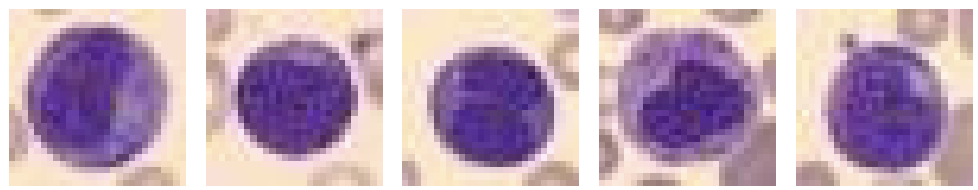
\includegraphics[width=\linewidth]{figures/immature-ranulocytes-class-3-1-row.png}
			\caption{Immature Granulocytes}
			\label{fig:methodA}
		\end{subfigure}
		\begin{subfigure}{\columnwidth}
			\centering
			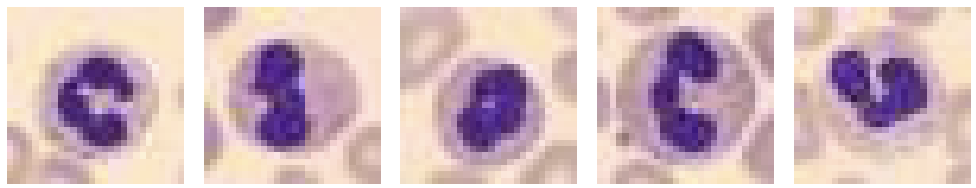
\includegraphics[width=\linewidth]{figures/neutrophil-class-6-1-row.png}
			\caption{Neutrophil}
			\label{fig:methodB}
		\end{subfigure}
		\caption{Representative BloodMNIST images. Immature granulocytes (a) exhibit a developing nucleus with limited segmentation, whereas neutrophils (b) display darker, multi-lobed connected nuclei.}
		\label{fig:bc-comparison}
	\end{figure}
	
	
	\begin{figure*}[t]
		\centering
		\begin{subfigure}[b]{0.32\textwidth}
			\centering
			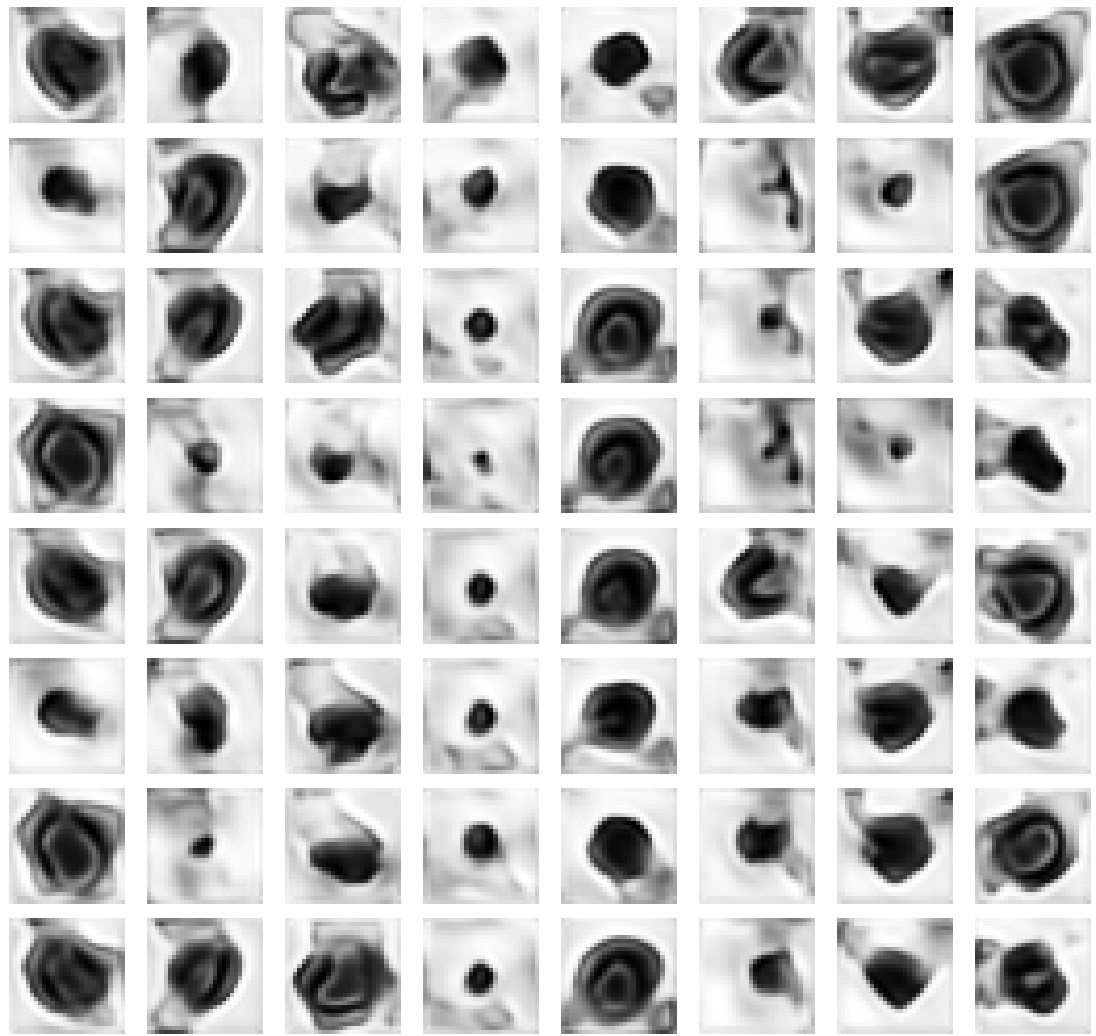
\includegraphics[width=\linewidth]{figures/blood-mnist-34k.png}
			\caption{Iteration 34k}
			\label{fig:blood-mnist-1}
		\end{subfigure}
		\hfill
		\begin{subfigure}[b]{0.32\textwidth}
			\centering
			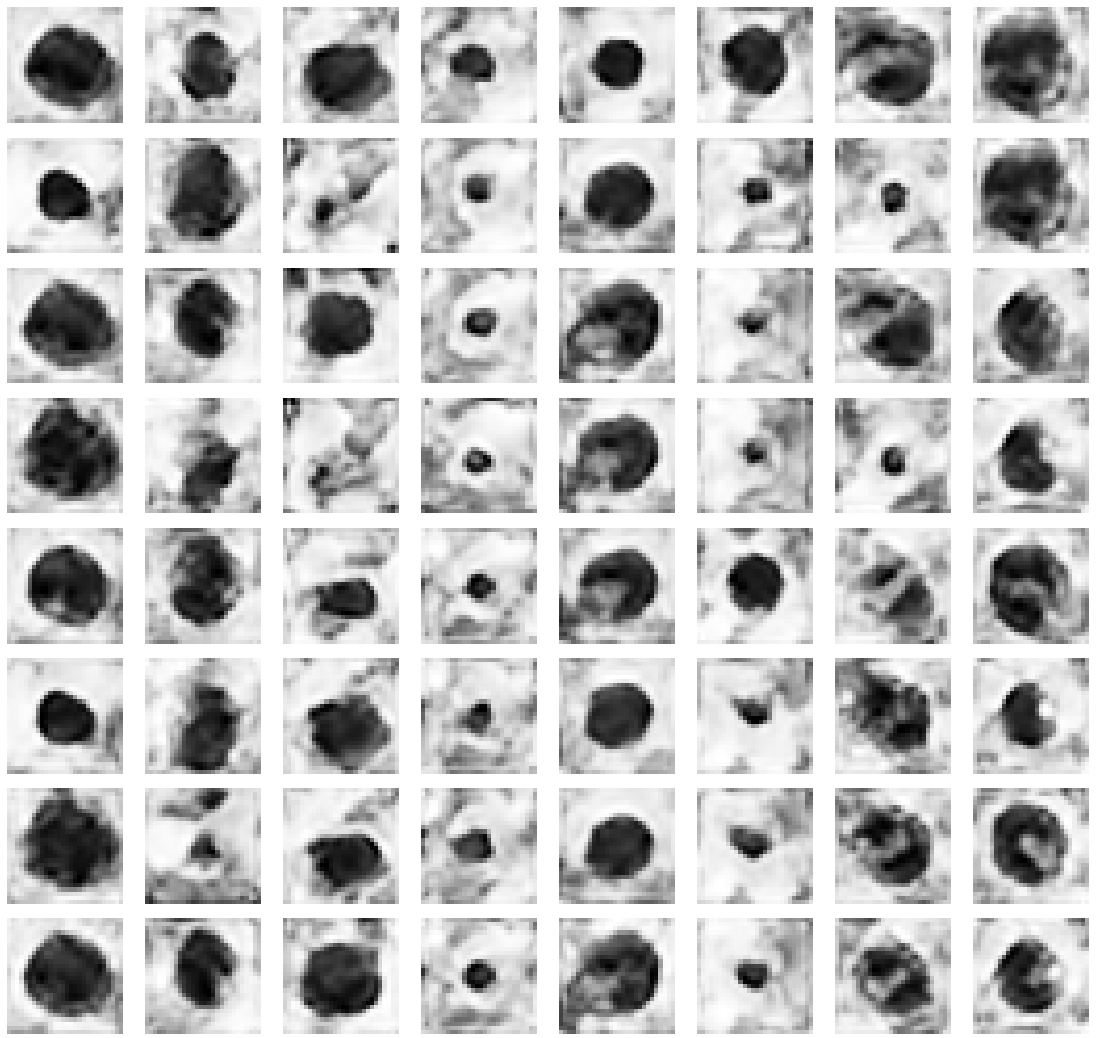
\includegraphics[width=\linewidth]{figures/blood-mnist-115k.png}
			\caption{Iteration 115k}
			\label{fig:blood-mnist-2}
		\end{subfigure}
		\hfill
		\begin{subfigure}[b]{0.32\textwidth}
			\centering
			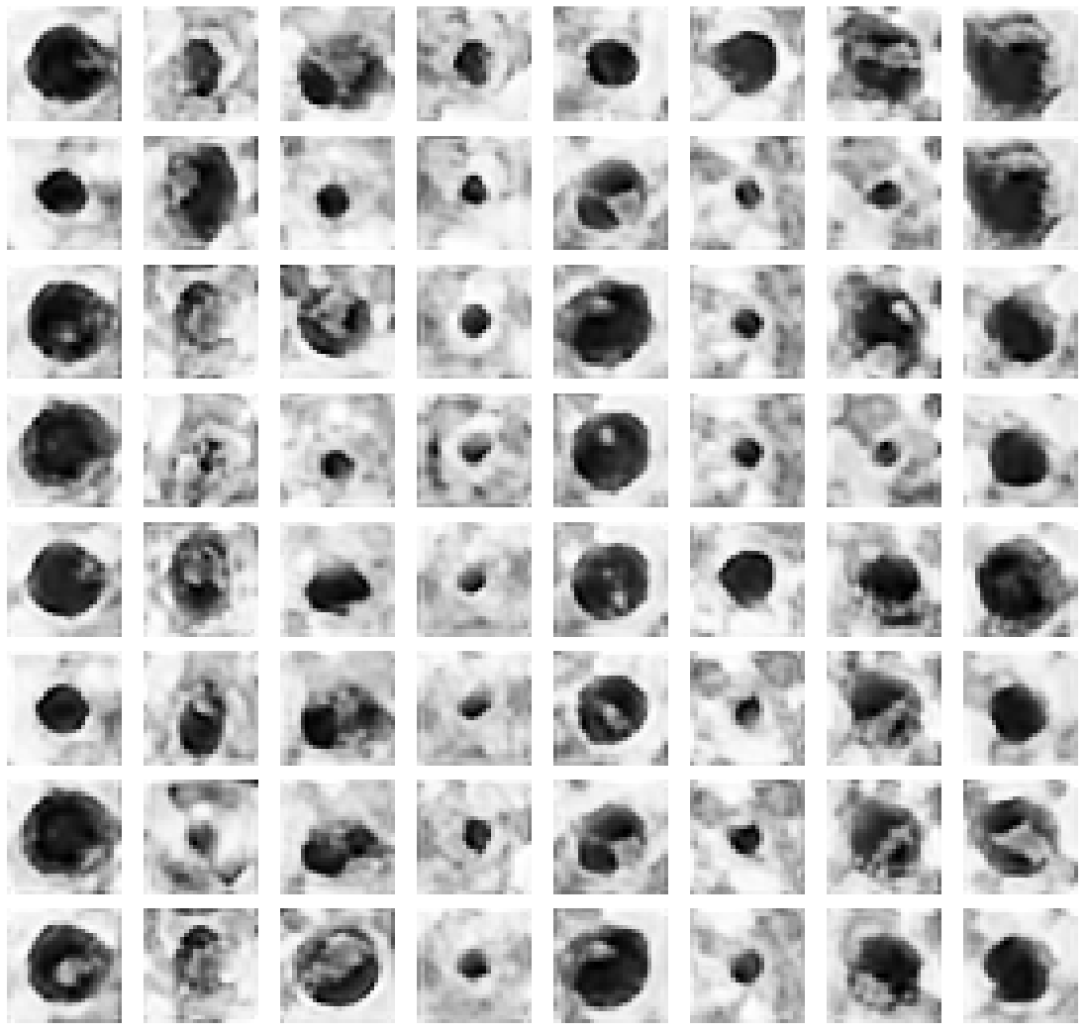
\includegraphics[width=\linewidth]{figures/blood-mnist-289k.png}
			\caption{Iteration 289k}
			\label{fig:blood-mnist-3}
		\end{subfigure}
		\caption{BloodMNIST same-run evaluation images at early, mid, and late checkpoints.}
		\label{fig:blood-mnist-combined}
	\end{figure*}
	
	Figure \ref{fig:bc-comparison} illustrates the challenge of the dataset for just two classes, the cell body and the nucleus. They vary in shape and scale, while several coarse visual factors remain shared. The primary discriminative signal is often concentrated in the nucleus morphology rather than in the overall cell outline.

	Figure \ref{fig:blood-mnist-combined} compares generated BloodMNIST images from the same run at iterations 34k, 115k, and 289k across all eight discrete codes.
	
	At 34k (Figure \ref{fig:blood-mnist-1}), the Generator already produces recognizable cell-like structures, but cell boundaries are still irregular and the internal morphology is largely shared across codes. Most columns contain a similar circular cell body and a broadly similar nucleus pattern. This suggests that the model has learned a generic leukocyte-like template before establishing strong code-specific specialization.
	
	By 115k (Figure \ref{fig:blood-mnist-2}), two qualitative improvements are visible. First, cell boundaries become rounder and more sharply defined. Second, the nuclei begin to differentiate across codes: some codes produce larger and darker nuclei, while others produce smaller or lighter internal structure. This corresponds to improved mutual-information quality and stronger within-code consistency. This indicates the onset of partial latent disentanglement.
	By 289k (Figure \ref{fig:blood-mnist-3}), the cells exhibit richer internal texture and more complex grayscale morphology than at either earlier checkpoint. The images are smoother and more artifact-free, and several codes show more varied nucleus fill and internal staining patterns. However, this late-stage improvement is primarily a refinement of a shared template family rather than a clean separation into distinct hematologic morphologies. In other words, the model continues to improve local realism and within-code variation, but the discrete codes still do not map cleanly onto the eight BloodMNIST classes. Late training therefore improves biological plausibility more than biological separation.
	Throughout training, the adversarial balance remains stable (\texttt{real\_fake\_loss} $\approx 0.56$--$0.59$), with no mode collapse or divergence observed. The model uses the same architecture and phased fitness schedule as the MNIST baseline, with the dataset adapted only through grayscale BloodMNIST inputs. Table~\ref{tab:blood_metrics} summarizes the corresponding training metrics.
	
	\begin{table}[b]
		\centering
		\caption{BloodMNIST training metrics for early, mid, and late checkpoints. $mi_{avg}$ denotes mutual information between discrete codes and generated images. $r_{\text{sense}}$ measures feature-space separation between code clusters. $r_{\text{intra}}$ measures within-code variation. ProtoCorr denotes the average correlation between code prototypes (lower is better separation). RFL denotes \texttt{real\_fake\_loss}.}
		\label{tab:blood_metrics}
		\begin{tabular}{lccccc}
			\toprule
			Iteration & $mi_{avg}$ & $r_{\text{sense}}$ & $r_{\text{intra}}$ & ProtoCorr & RFL \\
			\midrule
			34k  & 0.077 & 0.170 & 0.560 & 0.681 & 0.523 \\
			115k & 0.086 & 0.161 & 0.647 & 0.633 & 0.561 \\
			289k & 0.092 & 0.155 & 0.910 & 0.701 & 0.584 \\
			\bottomrule
		\end{tabular}
	\end{table}
	
	\section{Trust Relevance and Limitations}
	The architectural design of this HyperNet-InfoGAN is aligned with a core requirement of trustworthy synthetic medical imaging: latent control should be auditable, stable, and interpretable. In clinical settings, a user should be able to vary a generative factor in a controlled way and inspect whether the resulting changes remain medically plausible. 
	
	In this baseline, the combination of PGPE-based generator optimization, a backpropagation-trained discriminator, and an information-theoretic Q-head yields a stable adversarial training process for both the MNIST and BloodMNIST. On MNIST, the indirect encoding resolves duplicate-mode attractors that persisted indefinitely under direct-encoding, achieving full coverage of all ten digit classes. 
	
	On BloodMNIST, the same architecture and fitness schedule transfer without dataset-specific tuning, produces realistic grayscale cell morphologies with partial code separation. In both cases, the model avoids the severe collapse and artifact-heavy behavior observed in earlier direct-encoding runs. This suggests that indirect evolutionary search can support more reliable training dynamics in medically relevant image domains. At the same time, the BloodMNIST results expose an important limitation.
	
	Although the model achieves partial code separation, the discrete codes are not yet mapped to fully separated hematologic morphologies. The generator tends to express code differences through low-cost geometric factors such as cell size, nucleus position, and orientation within a narrow family of leukocyte-like templates. This indicates that mutual-information-driven disentanglement is not sufficient by itself to produce clinically meaningful variation. In other words, mathematical code separation does not necessarily imply biological separation. For clinical utility, future versions of the method will likely require morphology-aware objectives or priors, for example constraints such as nucleus-to-cytoplasm structure, nucleus shape, or class-consistent texture. This information can allow the learned latent codes to align more directly with medically-interpretable cell characteristics.
	
	\section{Conclusion}  This work demonstrates that replacing direct parameter evolution with a compact hypernetwork-based indirect encoding fundamentally changes the trainability of evolutionary InfoGAN models. On MNIST, the reduced searchspace (${\sim}$32k vs.\ $>$500k parameters) enables PGPE to resolve duplicate-mode attractors that were permanent failure states under direct-encoding. The same architecture and diversity-first fitness schedule transfer to BloodMNIST without modification, produced stable training and realistic cell morphologies. That is a necessary first step toward controllable synthetic medical image generation.
	The BloodMNIST baseline also reveals that static fitness functions, even with mutual-information objectives, remain vulnerable to geometric shortcuts in complex medical image distributions. Future work will address this gap between mathematical disentanglement and biological separation. The next step will integrate a CA layer in order to adaptively re-weight the evolutionary fitness landscape during training. This will support the use of morphology-aware priors to align latent codes with clinically meaningful structure.

	\bibliography{aaai2026}
	
\end{document}
